\documentclass[10pt]{beamer}
\usetheme[progressbar=frametitle]{metropolis}
\usepackage{booktabs}
\usepackage[scale=2]{ccicons}
\usepackage{pgfplots}
\usepgfplotslibrary{dateplot}
\hypersetup{
    colorlinks=true,
    linkcolor=blue,
    filecolor=magenta,      
    urlcolor=cyan,
}
 
\urlstyle{same}

\usepackage{xspace}
\newcommand{\themename}{\textbf{\textsc{metropolis}}\xspace}

\title{Study of Spontaneous and Acted Learned-Related Emotions Throught FER and GSR}
%\subtitle{going beyond IF and Scopus index (v2.0)}
\date{23 Oct 2018}
\author{Andres Mitre and Hugo Mitre-Hernandez}
%\author{Andres Mitre}

\institute{Human-Centered Computing Lab,\\
Center for Research in Mathematics (CIMAT),\\
Event: 11th Workshop on Intelligent Learning Environments (WILE), \\
Monterrey Institute of Technology and Higher Education (ITESM),\\
Guadalajara, Mexico.}
\titlegraphic{\hfill
\includegraphics[height=1.3cm]{Logo_con_CIMAT.png}}

\begin{document}
\maketitle

%\begin{frame}[standout]
%\begin{center}This material is licensed under a \href{http://creativecommons.org/licenses/by-sa/4.0/}{Creative Commons - Attribution 4.0 International License}\end{center}
%\begin{center}\ccby\end{center}
%\end{frame}


  
\begin{frame}{Agenda}
  \setbeamertemplate{section in toc}[sections numbered]
  \tableofcontents[hideallsubsections]
\end{frame}

\section{Introduction: scientific communication}

\begin{frame}{Introduction (1)}
There are several acted or spontaneous FER datasets related with learning activities.
	\begin{itemize}
    \item \caption{Lack of boredom and stress\footnote[frame]{%
    Lucey, P., Cohn, J.F., et al. The extended cohn-kanade dataset (ck+): A complete dataset for action unit and emotion- specified expression. In: Computer Vision and Pattern Recognition Workshops (CVPRW), 2010 IEEE Computer Society Conference on. pp. 94–101. IEEE (2010)}} \caption{\footnote[frame]{%
    Mavadati, S.M., Mahoor,et. al: Disfa: A spontaneous facial action intensity database. IEEE Transactions on Affective Computing 4(2), 151–160 (2013)}}
    \item Millions of Mult-Adds %(\textcolor{red}{test}).
	\end{itemize}
\end{frame}
 

\begin{frame}{Introduction (2)}
  Emotion
    \begin{itemize}
    \item terus menulis: dalam media formal maupun non formal,
    \item menggunakan indikator \emph{impact factor}, \emph{Scopus Indexing} dengan tidak berlebihan, serta memahami bahwa \emph{citation index} adalah sebuah indikator \emph{outcome}, bukan indikator proses,
    \item mengutamakan media \emph{open access} dan sajikan data mentah secara terbuka,
    \item mencoba menghasilkan artikel dalam Bahasa Inggris,
    \item memanfaatkan \emph{social media}.
  \end{itemize}
\end{frame}
  
  
\begin{frame}
	\metroset{block=fill}
  	\begin{exampleblock}{Pilihan di tangan kita.}
	\begin{itemize}
	\item Apakah akan menjadi akademia yang tertutup atau terbuka.
    \item Apakah kita akan menjalin jejaring luas atau puas dalam 'tempurung' saja.
    \item dan Apakah menjadi makhluk yang mensyukuri nikmat dan tidak kikir membagi ilmu atau sebaliknya.
	\end{itemize}
  \end{exampleblock}
\end{frame}
  
\begin{frame}{definitions}
	\metroset{block=fill}
    \begin{exampleblock}{scientific/scholarly communication according to \href{https://en.wikipedia.org/wiki/Science_communication}{Wikipedia}}
	\begin{itemize}
    \item refers to public communication presenting science-related topics to non-experts. 
    \item aims to generate support for scientific research or study, or to inform decision making, including political and ethical thinking. 
    \item emphasizes on explaining methods and findings.
    \end{itemize}
    \end{exampleblock}
\end{frame}

\begin{frame}{research cycle}
	\begin{figure}[!ht]
  	\centering
  	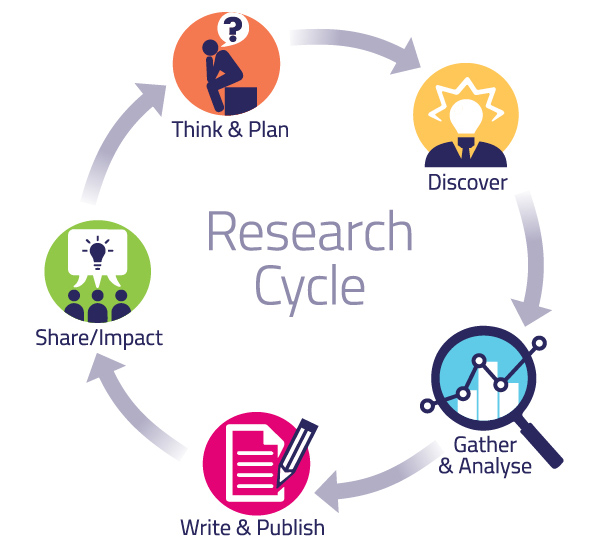
\includegraphics[width=3in]{research-cycle.jpg}
    \caption{\href{http://www.uh.edu/~qepsite/discovery/eDISCOVERY_Mentors_FAQs.htm}{Research cycle (Research resources: Edinburgh Napier Univ.}}
	\end{figure}
\end{frame}
  
\begin{frame}{so what is impact factor and why is it important?}
  \begin{quote}
  The journal Impact Factor is the average number of times articles from the journal published in the past two years have been cited in the JCR year. The Impact Factor is calculated by dividing the number of citations in the JCR year by the total number of articles published in the two previous years. (\href{admin-apps.webofknowledge.com/JCR/help/h_impfact.htm}{Thomson Reuters: Web of Science})
  \end{quote}
\end{frame}
  
\begin{frame}{so what is impact factor and why is it important?}
  Hence IF reflects:
      \begin{itemize}
      \item \textcolor{blue}{age}: the operational period of the medium (journal)
      \item \textcolor{blue}{visibility}: meaning older journals are read by more people than younger journals
      \item \textcolor{blue}{recognition}: meaning more citations
 	 \end{itemize}  
\end{frame}

\begin{frame}[standout]
    \begin{itemize}
	\item is it important? some would say \textbf{yes}
	\item does it apply to all of us? definitely \textbf{no}    
	\end{itemize}
\end{frame}

\begin{frame}{my citation index/H-index is high, what is good about it?}
   CI reflects:
     \begin{itemize}
     \item \textcolor{blue}{age}: old articles have higher chance to get more citations than recent ones,
     \item \textcolor{blue}{contextual}: articles match with certain issues will attract more readers,
     \item \textcolor{blue}{closed-calculation}: CI is calculated based on articles which are published in journals that include in the \href{http://isiknowledge.com/wos}{WoS} indexing database.
     \end{itemize}
\end{frame}


\begin{frame}{indexed by Scopus is important, why?}
	Indexed by Scopus means:
	\begin{itemize}
    \item journal/conference registration by journal/conference editorial, 
    \item selection by Scopus team based on Scopus criteria, 
    \item recognition (\textcolor{blue}{to some parties}).
	\end{itemize}
\end{frame}

\section{Related Works: Learn-Related approaches}

\begin{frame}{characteristics}
    \begin{exampleblock}{legacy scientific media characteristics}
	\textcolor{blue}{Closed-system}: readers (and even authors) have to be subscribed!
	\begin{itemize}
    \item \textcolor{blue}{closed data} (electronic supplementary data services are available with fee),
    \item \textcolor{blue}{blind peer-review} (pre publication)
    \item \textcolor{blue}{closed-loop distribution}, copyright transfer agreement
    \end{itemize}
    \end{exampleblock}
\end{frame}
  
\begin{frame}{example}
	Just go to \href{www.elsevier.com}{Elsevier}
\end{frame}

\section{Experiment: open science}

\begin{frame}{charactistics}
    \begin{exampleblock}{open science components \href{http://www.slideshare.net/Acceso2/introduction-to-open-science}{FOSTER 2015}}
	\begin{itemize}
    \item \href{http://opendatahandbook.org/guide/en/what-is-open-data/}{open data} 
    \item open methods (to endorse \href{https://en.wikipedia.org/wiki/Reproducibility}{reproducibility} and \href{https://publication2application.org/2014/06/09/replicability-in-research-and-practice/}{replicability})
    \item (using) open source software
    \item open access to research outputs
    \item \href{https://en.wikipedia.org/wiki/Open_peer_review}{open peer-review} (pre or post publication)
    \end{itemize}
    \end{exampleblock}
\end{frame}

\begin{frame}{example}
	\begin{itemize}
    \item \href{http://plosone.org/}{PLOS}
    \item \href{http://f1000research.com/}{F1000Research}
    \item \href{http://riojournal.com/}{RIO journal}
    \item \href{http://scienceopen.com/}{ScienceOpen}
    \item \href{http://thewinnower.com/}{The Winnower}
    \item \href{http://hydrol-earth-syst-sci-discuss.net/}{HESS}
    \item \href{http://www.nature.com/ncomms/index.html}{Nature Communications}
    \item etc more and more: go to \href{http://doaj.org/}{DOAJ} for more list
    \end{itemize}
\end{frame}


\begin{frame}{about that open access thingy}
	\begin{figure}[!ht]
  	\centering
  	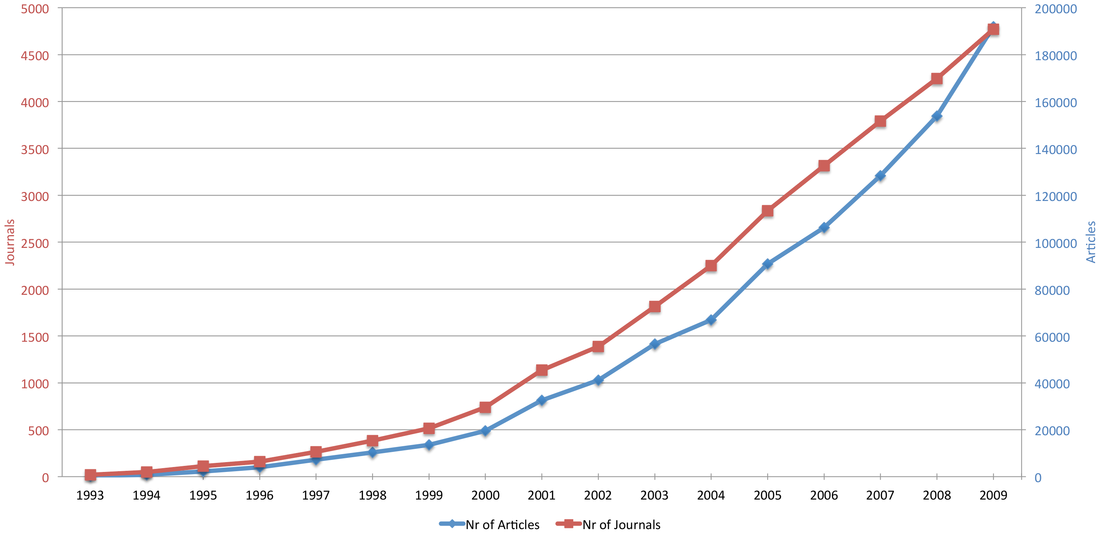
\includegraphics[width=3in]{Dev_oa.png}
    \caption{The development of open access}{\href{https://en.wikipedia.org/wiki/Open_access}{Wikipedia/Open Access}}
	\end{figure}
\end{frame}


\begin{frame}{about that open access thingy}
	\begin{figure}[!ht]
  	\centering
  	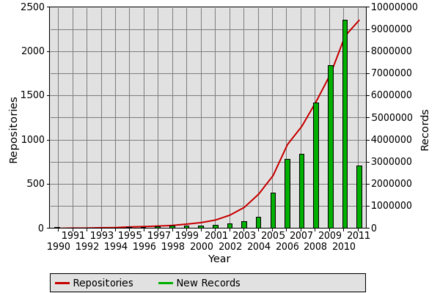
\includegraphics[width=3in]{self_archive_Roar2011.png}
    \caption{Number of self-archiving repositories and records}{\href{https://en.wikipedia.org/wiki/Registry_of_Open_Access_Repositories}{Wikipedia/Registry of Open Access Repositories}}
	\end{figure}
\end{frame}

\begin{frame}{about that open access thingy}
	\begin{figure}[!ht]
  	\centering
  	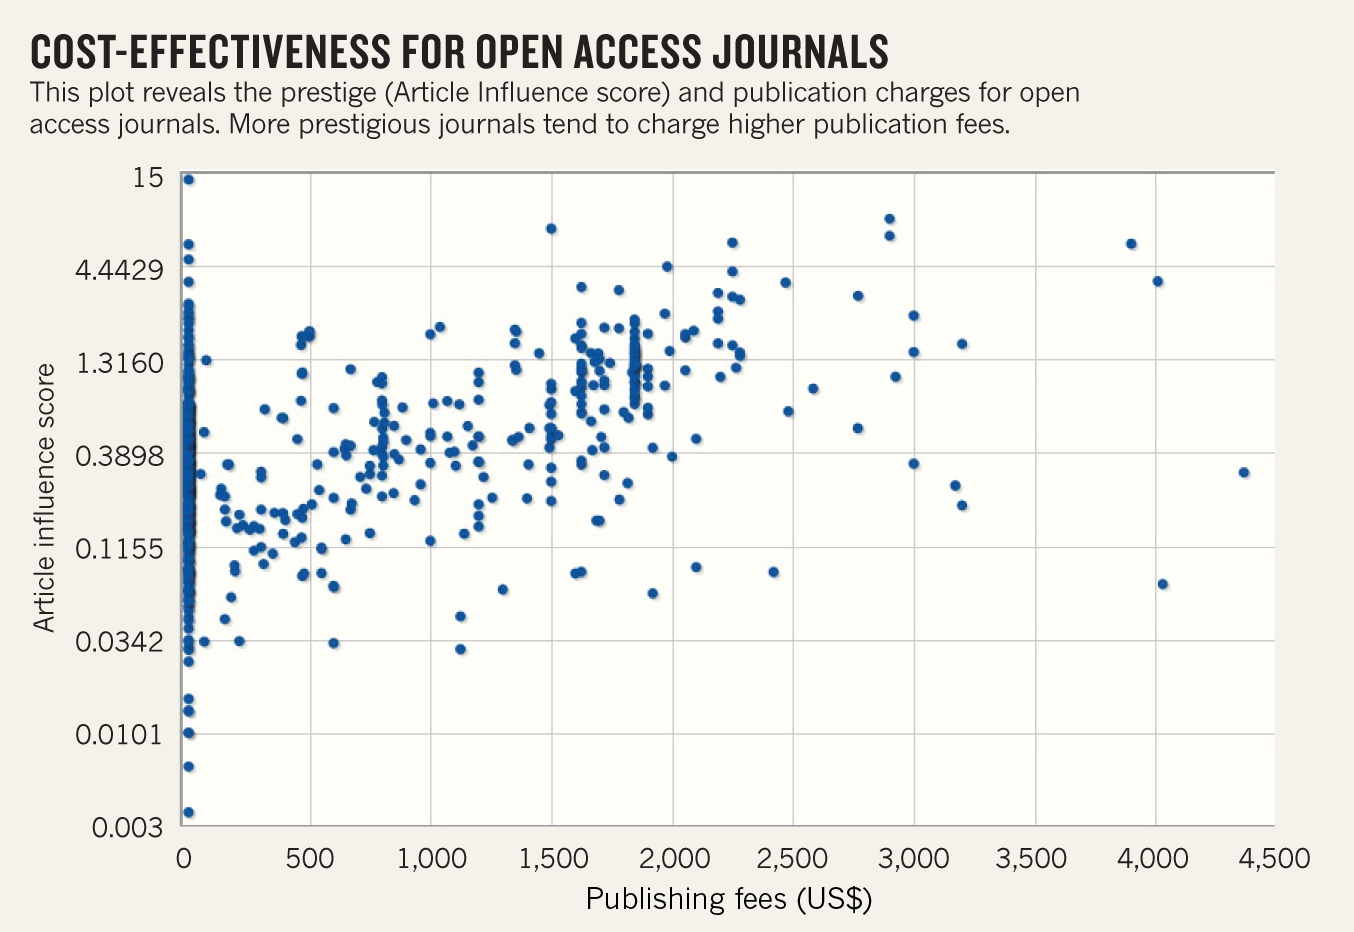
\includegraphics[width=3in]{Article_influence_chart.jpg}
    \caption{Journal APC vs reputation}{\href{http://www.nature.com/news/price-doesn-t-always-buy-prestige-in-open-access-1.12259}{Price doesn't always buy prestige in open access}}
	\end{figure}
\end{frame}

\begin{frame}{my example: what I am starting to do and keeping it as habit}
  \begin{itemize}
  	\item stage 1: research proposal
    \item stage 2: research implementation
    \item stage 3: report writing and publications
    \item stage 4: dissemination
    \item stage 5: data set management
  \end{itemize}
\end{frame}

\begin{frame}{stage 3: report writing and publications}
   \begin{itemize}
   \item make a report and upload it along with the data set to accessible repository (eg: 
   \href{www.figshare.com}{Figshare},
   \href{www.zenodo.org}{Zenodo}, or 
   \href{http://osf.io}{OSF}) or self archiving system,    
   \item cite the repository in your papers,
   \item post the repository on socmed (read \href{http://www.slideshare.net/flxlex/how-and-why-i-use-blogging?qid=19764e8a-1bdc-4878-b275-497c85cd664f&v=&b=&from_search=7}{How and why I use blogging}).
  \end{itemize}
\end{frame}
  
\begin{frame}{stage 3: report writing and publications}
   \begin{itemize}
   \item Where to publish?
   \item How much does it cost?
   \item Do we still have rights?
   		\begin{itemize}
  		\item open access vs conventional/legacy journals. 
    	\item problem with open access: \texttt{article publishing cost}
    	\item problem with legacy journals: \texttt{copyright transfer agreement}
  		\end{itemize}
  \end{itemize}
\end{frame}
  
\begin{frame}{stage 4: dissemination}
  \begin{itemize}
  	\item it's about how to increase impact: via \texttt{online visibility}
    \item what are the tools? You can try: \href{www.impactstory.org}{ImpactStory} or \href{www.growkudos.com}{GrowKudos} 
    \item how much does it cost? \texttt{Connection cost only}
  \end{itemize}
\end{frame}
  

\begin{frame}{scientific social media vs open access space}
  \begin{itemize}
  	\item is RG/Academia an open access space?
    \item answer: no, they're socmeds
    \item they offers archiving facilities in return of selling ads.
  \end{itemize}
\end{frame}
  
\section{Results and discussion}

\begin{frame}{further readings}

	A curated list of readings are also available on my Zenodo repository 
	\begin{itemize}
    \item Tennant, J., 2016, The open citation index, \href{http://blog.scienceopen.com/2016/02/the-open-citation-index/}{Blog Science Open}. 
    \item Pevatolo, M.C., 2016, Private spaces, public science?
Open access and academic social media, \url{https://t.co/ublvRi9ScM}
    \item Kim, H., 2015, How to index journal in Scopus and WoS, (\href{https://zenodo.org/deposit/125607/}{Zenodo repo})
    \item Broch, E., 2011, Journal Impact factors: what they mean, what they don't mean, and why you should care, Princeton blogs (\href{https://zenodo.org/deposit/125607/}{Zenodo repo})
    \end{itemize}
    
\end{frame}

\begin{frame}{further readings}
\begin{itemize}
    \item \href{http://theconversation.com/busting-the-top-five-myths-about-open-access-publishing-14792}{The Conversations:
Busting the top five myths about open access publishing
}
    \item \href{http://www.nature.com/news/price-doesn-t-always-buy-prestige-in-open-access-1.12259}{Nature: Price doesn't always buy prestige in open access}
    \item \href{https://en.wikipedia.org/wiki/Registry_of_Open_Access_Repositories}{Wikipedia/Registry of Open Access Repositories}
    \item \href{https://en.wikipedia.org/wiki/Open_access}{Wikipedia/Open Access}
    \item \href{http://www.slideshare.net/flxlex/how-and-why-i-use-blogging?qid=19764e8a-1bdc-4878-b275-497c85cd664f&v=&b=&from_search=7}{How and why I use blogging}
    \item more readings online.
\end{itemize}
    
\end{frame}

\section{Conclusion / Future work}

\begin{frame}{take home notes}

\begin{center}science is about:\end{center}

\begin{center}
\begin{enumerate}
	\item \textcolor{blue}{honesty} in researching the problem
	\item \textcolor{blue}{bravery} in publishing the results 
    \item \textcolor{blue}{big heart} in getting feedback 
\end{enumerate}
\end{center}

\end{frame}

\begin{frame}[standout]

\begin{center}
\LaTeX  source is available at \\
\href{www.overleaf.com/5507974mcbqsc}{Overleaf}
\end{center}

\begin{center}
Slides/decks in pdf is available at \\
\href{www.slideshare.net/d_erwin_irawan}{Slideshare}
\end{center}

\end{frame}

\begin{frame}[standout]
\begin{center}This material is licensed under a \href{http://creativecommons.org/licenses/by-sa/4.0/}{Creative Commons - Attribution 4.0 International License}\end{center}
\begin{center}\ccby\end{center}
\end{frame}

\begin{frame}{about me}
  \begin{itemize}
	\item place/date of birth: Surabaya/17 April 1976
    \item education: Teknik Geologi ITB: S1 ('94-'98), S2 ('99-'01), S3 ('05-'09)
    \item media: twitter \href{www.twitter.com/dasaptaerwin}{@dasaptaerwin}, facebook Dasapta Erwin Irawan
  \end{itemize}
\end{frame}

\end{document}
